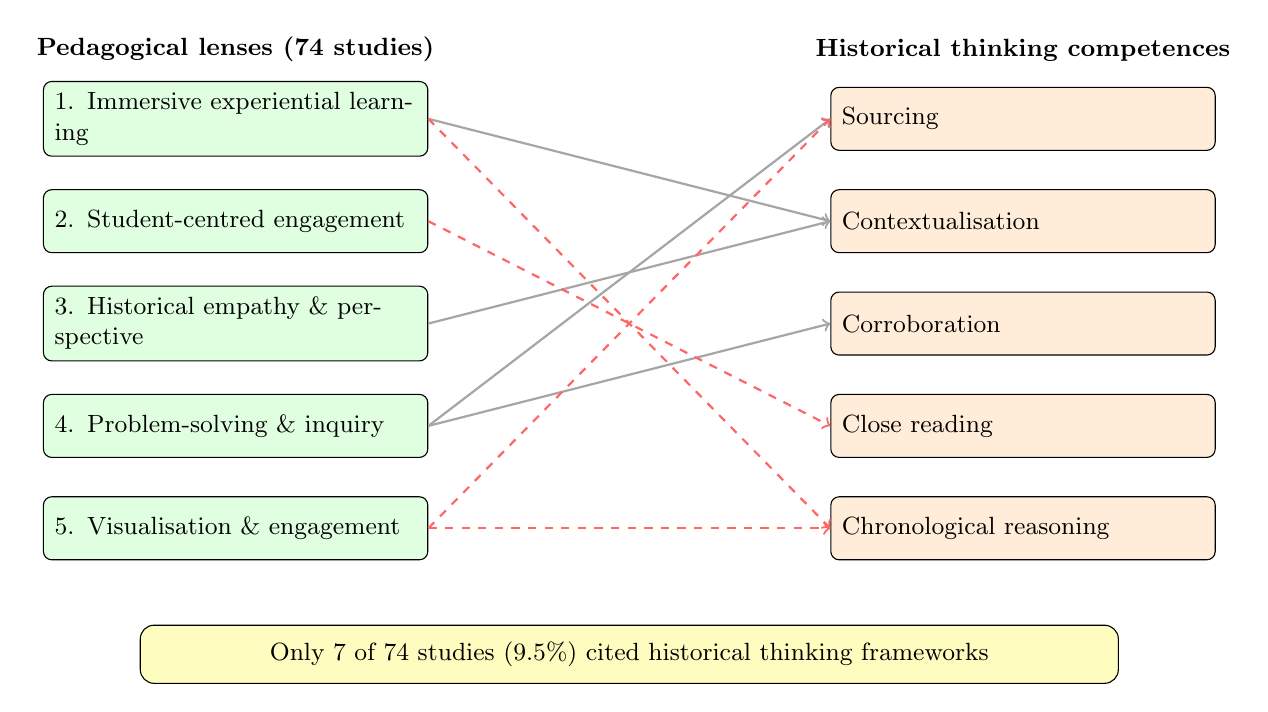
\begin{tikzpicture}[
  every node/.style={font=\small},
  pedbox/.style={rectangle, draw, rounded corners=3pt, fill=green!12,
    minimum width=4.8cm, minimum height=0.8cm, text width=4.6cm,
    align=left, font=\small, inner sep=4pt},
  histbox/.style={rectangle, draw, rounded corners=3pt, fill=orange!15,
    minimum width=4.8cm, minimum height=0.8cm, text width=4.6cm,
    align=left, font=\small, inner sep=4pt},
  colhead/.style={font=\small\bfseries, anchor=south},
  callout/.style={rectangle, draw, rounded corners=5pt, fill=yellow!25,
    font=\small, inner sep=6pt, text width=12cm, align=center},
]

% Column headers
\node[colhead] at (0, 0.6) {Pedagogical lenses (74 studies)};
\node[colhead] at (10, 0.6) {Historical thinking competences};

% Left column: Pedagogical lenses
\node[pedbox] (P1) at (0, 0) {1. Immersive experiential learning};
\node[pedbox] (P2) at (0, -1.3) {2. Student-centred engagement};
\node[pedbox] (P3) at (0, -2.6) {3. Historical empathy \& perspective};
\node[pedbox] (P4) at (0, -3.9) {4. Problem-solving \& inquiry};
\node[pedbox] (P5) at (0, -5.2) {5. Visualisation \& engagement};

% Right column: Wineburg's historical thinking
\node[histbox] (H1) at (10, 0) {Sourcing};
\node[histbox] (H2) at (10, -1.3) {Contextualisation};
\node[histbox] (H3) at (10, -2.6) {Corroboration};
\node[histbox] (H4) at (10, -3.9) {Close reading};
\node[histbox] (H5) at (10, -5.2) {Chronological reasoning};

% Solid arrows: established connections
\draw[->, thick, gray!70] (P1.east) -- (H2.west);
\draw[->, thick, gray!70] (P3.east) -- (H2.west);
\draw[->, thick, gray!70] (P4.east) -- (H1.west);
\draw[->, thick, gray!70] (P4.east) -- (H3.west);

% Dashed arrows: underexplored alignments
\draw[->, dashed, red!60, thick] (P1.east) -- (H5.west);
\draw[->, dashed, red!60, thick] (P2.east) -- (H4.west);
\draw[->, dashed, red!60, thick] (P5.east) -- (H1.west);
\draw[->, dashed, red!60, thick] (P5.east) -- (H5.west);

% Callout box
\node[callout] at (5, -6.8)
  {Only 7 of 74 studies (9.5\%) cited historical thinking frameworks};

\end{tikzpicture}
